\documentclass[11pt]{article}

\usepackage[utf8]{inputenc}
\usepackage{hyperref}
\usepackage{graphicx}

\title{ Compulsory Assignment 1}
\author{ Petter Jakub Økland - 223073\\
Eivind Norling - 267792}

\begin{document}
\maketitle

\section{The Karate Club Network}
\subsection{}
\begin{figure}
  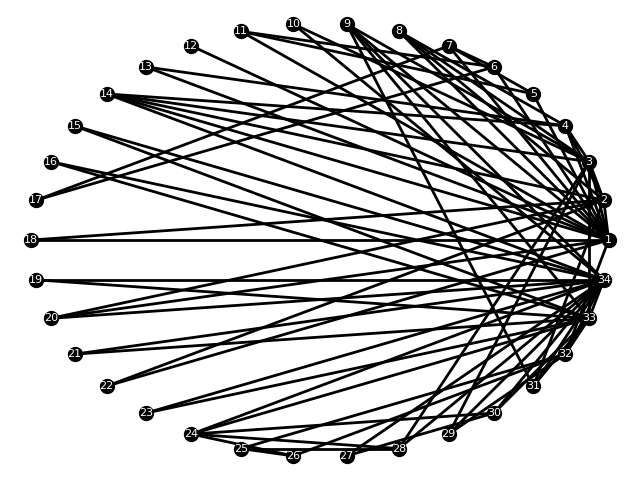
\includegraphics[width=\linewidth]{Figure_1.png}
  \caption{A graph.}
  \label{fig:graph model}
\end{figure}

Figure \ref{fig:graph model} shows a graph.

\subsection{}
Zachary\cite{Zachary} analyzes the splintering of a karate club into two different organizations
over a dispute over lessen fees. He lists several reasons for formalizing this fission
process into a mathematical model, the most important perhaps being that the model is
new to anthropology.\\
\\
His analysis shows how the flow of political information predicts the two opposing
factions' increasingly divergent views and strategy ultimately leading to a fission
as information flow between factions becomes increasingly hampered by a bottleneck
of information between them.\\
\\
Beyond just club meetings, shared perceptions on the nature of the club communicated
in the friendship network was unable to become reconciled accross factional boundraries.
An organizational and ideological feedback relationship -- a vicious cycle-- wherein the
strategy of the factions increasingly intensified the ideological divide while threatening
the organizational basis for the network's existence itself made the fission all but
inevitable.\\
\\
The form of this analysis can be applied to more than just the karate club, extending to
analysis of communication patterns in small groups in general due to the inherency of the
the feature of the minimum cut in a capacitated network in this mathematical model, which
is what made this model quite new to anthropology at the time. Whenever the existence of
a unique minimum cut in a capacitated network can be established, it will under certain
conditions (here communication of club meetings) result in a barrier to group unity which
can end up in a group fission.

\section{}
Running the following functions yielded the following results:\\
\\
degree\_centrality(G)\\
1: 0.48484848484848486, 2: 0.2727272727272727, 3: 0.30303030303030304,
4: 0.18181818181818182, 5: 0.09090909090909091, 6: 0.12121212121212122,
7: 0.12121212121212122, 8: 0.12121212121212122, 9: 0.15151515151515152,
10: 0.06060606060606061, 11: 0.09090909090909091, 12: 0.030303030303030304,
13: 0.06060606060606061, 14: 0.15151515151515152, 15: 0.06060606060606061,
16: 0.06060606060606061, 17: 0.06060606060606061, 18: 0.06060606060606061,
19: 0.06060606060606061, 20: 0.09090909090909091, 21: 0.06060606060606061,
22: 0.06060606060606061, 23: 0.06060606060606061, 24: 0.15151515151515152,
25: 0.09090909090909091, 26: 0.09090909090909091, 27: 0.06060606060606061,
28: 0.12121212121212122, 29: 0.09090909090909091, 30: 0.12121212121212122,
31: 0.12121212121212122, 32: 0.18181818181818182, 33: 0.36363636363636365,
34: 0.5151515151515151
\\\\
betweenness\_centrality(G)\\
1: 0.43763528138528146, 2: 0.053936688311688304, 3: 0.14365680615680618,
4: 0.011909271284271283, 5: 0.0006313131313131313, 6: 0.02998737373737374,
7: 0.029987373737373736, 8: 0.0, 9: 0.05592682780182781, 10: 0.0008477633477633478,
11: 0.0006313131313131313, 12: 0.0, 13: 0.0, 14: 0.04586339586339586, 15: 0.0,
16: 0.0, 17: 0.0, 18: 0.0, 19: 0.0, 20: 0.03247504810004811, 21: 0.0, 22: 0.0,
23: 0.0, 24: 0.017613636363636363, 25: 0.0022095959595959595, 26: 0.0038404882154882154,
27: 0.0, 28: 0.02233345358345358, 29: 0.0017947330447330447, 30: 0.0029220779220779218,
31: 0.014411976911976909, 32: 0.13827561327561325, 33: 0.145247113997114, 34: 0.30407497594997596
\\\\
closeness\_centrality(G)\\
1: 0.5689655172413793, 2: 0.4852941176470588, 3: 0.559322033898305,
4: 0.4647887323943662, 5: 0.3793103448275862, 6: 0.38372093023255816,
7: 0.38372093023255816, 8: 0.44, 9: 0.515625, 10: 0.4342105263157895,
11: 0.3793103448275862, 12: 0.36666666666666664, 13: 0.3707865168539326,
14: 0.515625, 15: 0.3707865168539326, 16: 0.3707865168539326, 17: 0.28448275862068967,
18: 0.375, 19: 0.3707865168539326, 20: 0.5, 21: 0.3707865168539326,
22: 0.375, 23: 0.3707865168539326, 24: 0.39285714285714285, 25: 0.375,
26: 0.375, 27: 0.3626373626373626, 28: 0.4583333333333333, 29: 0.4520547945205479,
30: 0.38372093023255816, 31: 0.4583333333333333, 32: 0.5409836065573771, 33: 0.515625, 34: 0.55
\\\\
average\_clustering(G)\\
0.5706384782076823
\\\\
connectivity.local\_edge\_connectivity(G, 1, 34)\\
10\\
\\\\
As can be seen bla bla.

\section{Polarized blogging about climate change}


\section{The psychology of social media}


\pagebreak
\bibliography{references.bib}
\bibliographystyle{ieeetr}

\end{document}
